下の図はGoが実現するWebサービスの作業モードのプロセス図です

\begin{figure}[H]
  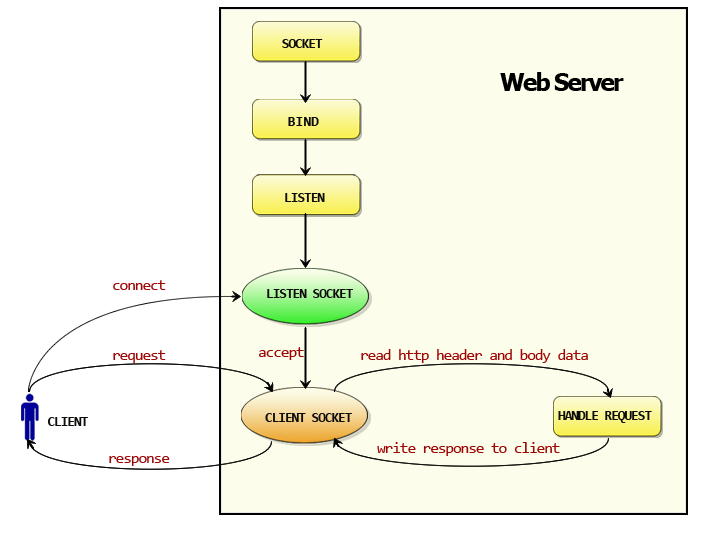
\includegraphics[width=14cm]{3.3.http.png}
   \label{図3.9}
   \caption{httpパッケージの実行フロー}
\end{figure}

\begin{enumerate}
  \item Listen Socketを作成し、指定したポートを監視します。クライアントのリクエストを待ちます。
  \item Listen Socketはクライアントのリクエストを受け付けます。Client Socketを得ると、Client Socketを通じてクライアントと通信を行います。
  \item クライアントのリクエストを処理します。まず、Client SocketからHTTPリクエストのプロトコルヘッダを読み取り、もしPOSTメソッドであれば、クライアントが入力するデータをさらに読み取るかもしれません。その後対応するhandlerがリクエストを処理します。handlerがクライアントの要求するデータを準備し終えたら、Client Socketを通じてクライアントに書き出します。
\end{enumerate}

この全体のプロセスでは3つの問題についてだけ理解しておけば構いません。これはまたGoがいかにしてWebを実行するのかということを知るという意味です。

\begin{itemize}
  \item どのようにポートを監視するか?
  \item クライアントのリクエストをどのように受け付けるか?
  \item handlerにどのように受け渡すか?
\end{itemize}

前の節のコードではGoは関数\texttt{ListenAndServe}を通してこれらの事を処理していました。ここでは実はこのように処理しています:serverオブジェクトを初期化します。その後\texttt{net.Listen("tcp", addr)}をコールします。つまり、低レイヤでTCPプロトコルを用いてサービスを立ち上げます。その後我々が設定したポートを監視します。

下のコードはGoのhttpパッケージのソースコードから引用したものです。下のコードで全体のHTTP処理プロセスを見ることができます。

\begin{lstlisting}[numbers=none]
func (srv *Server) Serve(l net.Listener) error {
    defer l.Close()
    var tempDelay time.Duration
                  // how long to sleep on accept failure
    for {
        rw, e := l.Accept()
        if e != nil {
            if ne, ok := e.(net.Error); ok && ne.Temporary() {
                if tempDelay == 0 {
                    tempDelay = 5 * time.Millisecond
                } else {
                    tempDelay *= 2
                }
                if max := 1 * time.Second; tempDelay > max {
                    tempDelay = max
                }
                log.Printf("http: Accept error: %v; retrying in %v",
                           e, tempDelay)
                time.Sleep(tempDelay)
                continue
            }
            return e
        }
        tempDelay = 0
        c, err := srv.newConn(rw)
        if err != nil {
            continue
        }
        go c.serve()
    }
}
\end{lstlisting}

監視した後どのようにしてクライアントのリクエストを受け取るのでしょうか?上のコードではポートの監視を実行後、\texttt{srv.Serve(net.Listener)}関数をコールしています。この関数はクライアントのリクエスト情報を処理しています。この関数では\texttt{for\{\}}が置かれており、まずListenerを通じてリクエストを受け取った後、Connを作成します。最後に単独のgoroutineを開きます。このリクエストのデータを引数としてこのconnに渡します。:\texttt{go c.serve()}。これはマルチスレッドを行なっています。ユーザが行うリクエストはすべて真新しいgoroutineの上で行われ、互いに影響しません。

ではいかにして具体的に目的の関数でリクエストを処理するように振り分けるのでしょうか?connはまずrequestを解析します:\texttt{c.readRequest()}、その後目的のhandlerを取得します:\texttt{handler := sh.srv.Handler}、つまり、我々がさきほど\texttt{ListenAndServe}をコールした時、その2つ目の引数です。前の例でnilを渡したのですが、これは空ということです。デフォルトで\texttt{handler = DefaultServeMux}を取得します。この変数は一体何に使われるのでしょうか?そうです。この変数はルータです。これはマッチするurlを対応するhandler関数にリダイレクトするために用いられます。我々はこれを設定したでしょうか?ええ。我々がコールしたコードのいの一番で\texttt{http.HandleFunc("/", sayhelloName)}をコールしたじゃないですか。これは\texttt{/}をリクエストするルートのルールを登録します。urlが"/"をリクエストした場合、ルートは関数sayhelloNameにリダイレクトします。DefaultServeMuxはServeHTTPメソッドをコールします。このメソッド内では実はsayhelloName本体をコールしています。最後にresponseの情報を入力することで、クライアントにフィードバックを返します。

全体のフローの詳細は以下の図の通りです:

\begin{figure}[H]
  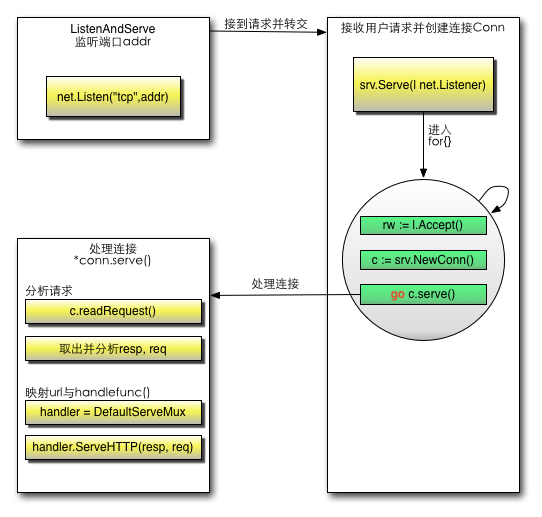
\includegraphics[width=14cm]{3.3.illustrator.png}
   \label{図3.10}
   \caption{http接続の処理フロー}
\end{figure}

ここに来て我々は3つの問題に対して全て解答を得ました。Goが如何にWebを走らせるか、すでに基本的なことは理解されたのではないでしょうか?
